\chapter{复合系统、纠缠与单态}

\lectureoverview{关于光子发射的问题揭示了量子事件与其系综平均之间的区别。这一区别自然引向测量、坍缩，以及将系统与其仪器一并处理的必要性。因此我们构造两个系统的张量积态空间，专门讨论两个自旋的情形，区分乘积态与纠缠态，并将每个单自旋可观测量嵌入复合空间。单态随后提供了决定性的例子：每个自旋在局部都是无偏振的，然而相等的分量却完全反关联。其与基无关的形式为贝尔定理以及非经典关联与超光速信号传递之间的区分奠定了基础。}

\section{叠加自旋的离散跃迁}

从一个处于沿\(z\)轴方向的磁场中的自旋开始。在\(\hbar=1\)的单位制下，
\begin{equation}
H=\frac{\omega}{2}\sigma_z,
\qquad
E_+=+\frac{\omega}{2},
\qquad
E_-=-\frac{\omega}{2}.
\label{eq:l6-spin-hamiltonian}
\end{equation}
两个能级之间的间隔为
\begin{equation}
\Delta E=E_+-E_-=\omega.
\label{eq:l6-energy-gap}
\end{equation}
当辐射场被纳入考虑时，处于上能级的自旋可能落到下能级并发射一个能量为\(\omega\)的光子。已经处于下能级的自旋则没有更低的自旋态可供其辐射跃迁。

\begin{figure}[htbp]
\centering
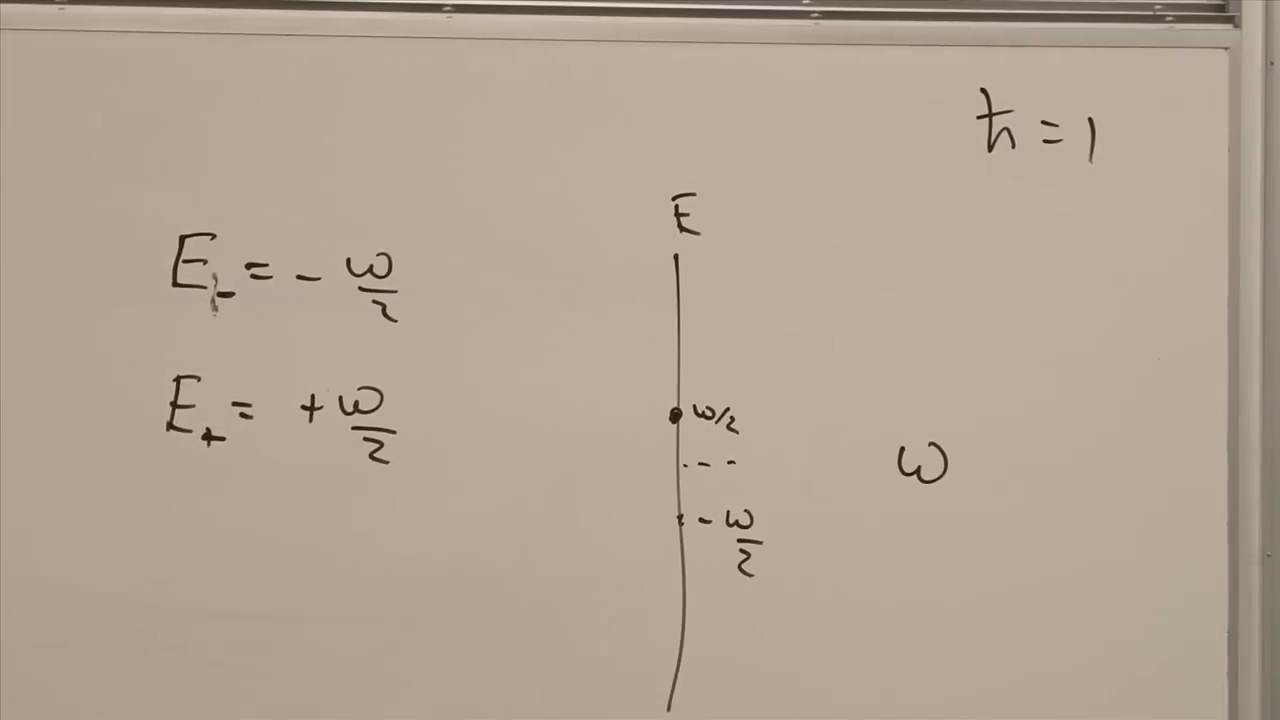
\includegraphics[width=0.86\textwidth]{lecture_06_figure_01.png}
\caption{两个自旋能级及其间隔\(\omega\)，其中\(\hbar=1\)。}
\lectureframe{00:02:35}
\end{figure}

微妙的情形是横向制备的自旋。经典磁性转子具有连续变化的能量，正比于其与磁场夹角的余弦。它以角频率\(\omega\)进动，以同一频率辐射，并逐渐落向其最小能量取向。总辐射能量连续地依赖于初始角度：初始水平的转子释放的能量是初始处于顶端者的一半。

量子力学仅将那个经典答案保留为平均值。写出
\begin{equation}
\ket{\psi}=\alpha\ket{u}+\beta\ket{d},
\qquad
|\alpha|^2+|\beta|^2=1,
\label{eq:l6-superposed-spin}
\end{equation}
其中\(\ket{u}\)和\(\ket{d}\)分别是上、下能量本征态。上分量可以衰变；下分量不能。因此
\begin{equation}
P(\text{one photon})=|\alpha|^2,
\qquad
P(\text{no photon})=|\beta|^2.
\end{equation}
如果发射了一个光子，其能量就是完整的能级间距\(\omega\)，而不是它的一部分。平均发射能量仍然是
\begin{equation}
\expect{E_{\rm emitted}}=|\alpha|^2\omega.
\end{equation}
对于沿\(x\)方向的自旋，\(|\alpha|^2=|\beta|^2=1/2\)，因此平均值为\(\omega/2\)。每个单独事件仍然要么产生一个能量为\(\omega\)的光子，要么不产生光子。连续的经典结果属于系综平均；离散性属于每个事件。

\begin{classroomqa}
\audiencequestion{被吸收的光子必须多精确地匹配能级间距？}
\lecturerresponse{共振具有有限的线宽。如果激发态的寿命为\(\tau\)，其特征能量宽度约为\(\Delta E\sim\hbar/\tau\)。较大的磁偶极矩通常与辐射场耦合更强，缩短寿命，并展宽谱线。这就是能量-时间不确定关系在与不稳定能级相关的形式下的体现。}
\end{classroomqa}

\begin{classroomqa}
\audiencequestion{光子发射本身能否充当测量自旋的仪器？}
\lecturerresponse{它可以揭示是否发生了衰变，但它并不是此处所需的理想可重复测量模型。对自旋分量的测量应当使自旋处于与所记录值相关联的本征态。而衰变则把每个已发射的分支都驱至下能级，因此它并非简单地记录两个可能的输入值同时保持其对应的本征态。}
\end{classroomqa}

\section{坍缩与复合系统的必要性}

在干预之间，孤立态按Schr\"odinger方程演化。测量通常被表述为一条附加规则。设\(L\)具有正交归一的本征矢\(\ket{\lambda_i}\)，并展开
\begin{equation}
\ket{\psi}=\sum_i\alpha_i\ket{\lambda_i},
\qquad
L\ket{\lambda_i}=\lambda_i\ket{\lambda_i}.
\label{eq:l6-measurement-expansion}
\end{equation}
一次测量以概率\(|\alpha_k|^2\)给出一个值\(\lambda_k\)，此后态为
\begin{equation}
\ket{\psi}\longrightarrow\ket{\lambda_k}.
\label{eq:l6-collapse}
\end{equation}
其他分量从测量后描述中的消失称为坍缩。

\begin{figure}[htbp]
\centering
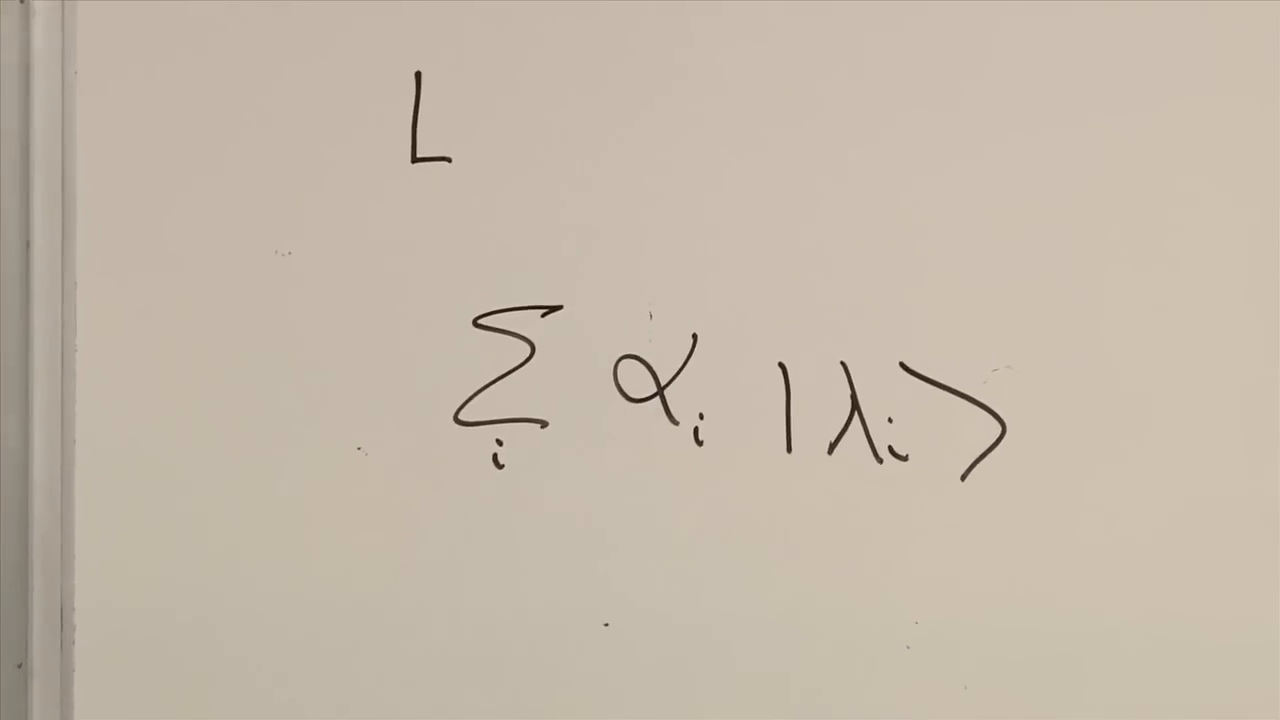
\includegraphics[width=0.84\textwidth]{lecture_06_figure_02.png}
\caption{一个在可观测量\(L\)的本征基中展开的态，在某个结果被选出之前。}
\lectureframe{00:12:35}
\end{figure}

\begin{classroomqa}
\audiencequestion{坍缩规则有什么问题？}
\lecturerresponse{作为预测测量结果的操作规则，它没有任何问题。概念上的张力在于，仪器本身也是一个物理系统。如果对象和仪器都服从量子力学，为什么它们的相互作用还需要在幺正的Schr\"odinger演化之外附加第二条动力学定律？此处采取的途径是将对象和仪器描述为一个更大的量子系统。}
\end{classroomqa}

系统与仪器之间那条分明的边界是历史争论的一个核心问题。我们不是通过断言来平息那场争论，而是先学习量子系统如何被组合。一旦有了组合后的态空间，测量就可以作为使系统与仪器相关联的一种相互作用来研究。因此，直接的数学问题是：
\begin{quote}
给定两个量子系统，整体的态空间是什么？
\end{quote}

\section{张量积态空间}

称这两个系统为\(A\)和\(I\)，其希尔伯特空间分别为\(\mathcal S_A\)和\(\mathcal S_I\)。它们的复合空间是
\begin{equation}
\mathcal S_{AI}=\mathcal S_A\otimes\mathcal S_I.
\label{eq:l6-tensor-space}
\end{equation}
为这两个因子各选一组正交归一基\(\{\ket{a}\}\)和\(\{\ket{i}\}\)。将第一个系统的每个基矢量与第二个系统的每个基矢量配对：
\begin{equation}
\ket{a}\otimes\ket{i}\equiv\ket{a\,i}.
\end{equation}
若因子空间的维数分别为\(D_A\)和\(D_I\)，则
\begin{equation}
\dim\mathcal S_{AI}=D_A D_I.
\end{equation}
内积按因子分解，
\begin{equation}
\braket{b\,j}{a\,i}
=\braket{b}{a}\braket{j}{i}
=\delta_{ba}\delta_{ji}.
\label{eq:l6-tensor-inner-product}
\end{equation}
因此，只要任一子系统的标签不同，两个复合基态就正交。

\begin{figure}[htbp]
\centering
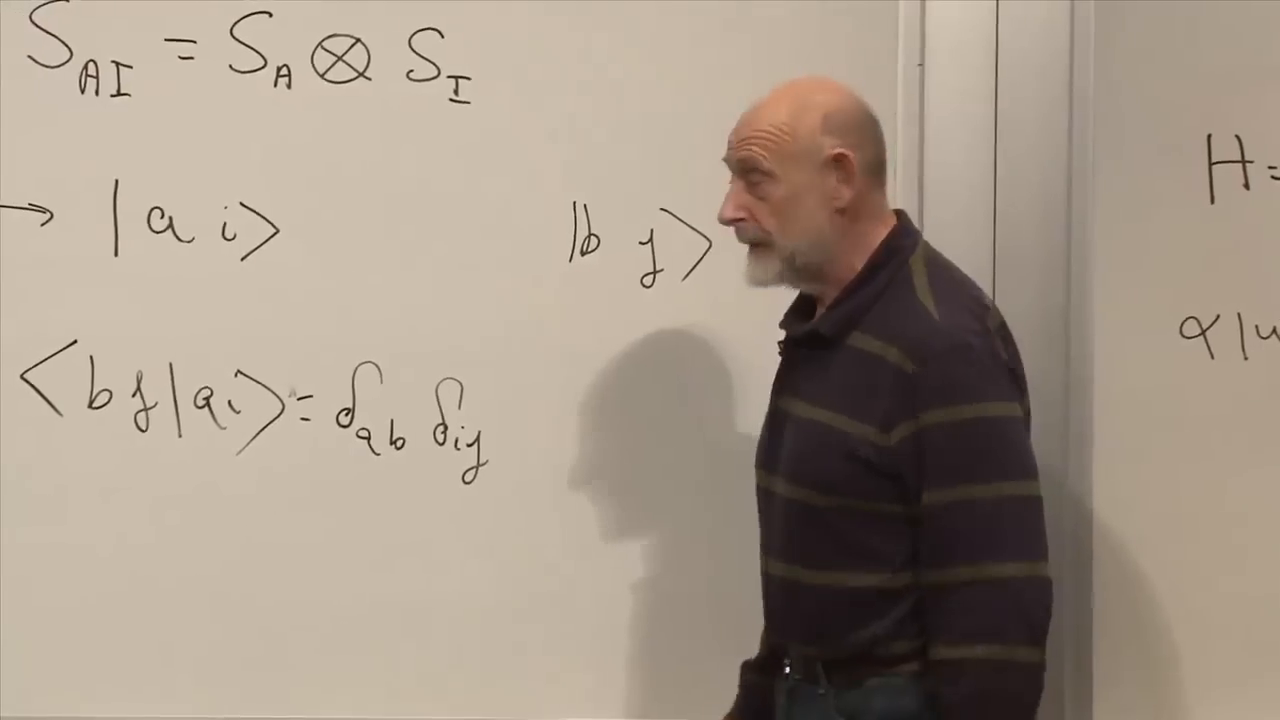
\includegraphics[width=0.86\textwidth]{lecture_06_figure_03.png}
\caption{分离的态空间、它们的张量积以及配对的正交归一基。}
\lectureframe{00:24:05}
\end{figure}

这些配对的基矢量并不构成整个空间。它们的完全线性张成是：
\begin{equation}
\ket{\Psi}=\sum_{a,i}c_{ai}\ket{a\,i},
\qquad
\sum_{a,i}|c_{ai}|^2=1.
\label{eq:l6-general-tensor-state}
\end{equation}

\begin{classroomqa}
\audiencequestion{\(\ket{a}\)和\(\ket{i}\)是任意矢量吗？}
\lecturerresponse{这里它们是所选正交归一基的成员。任一因子中都可以使用任意正交归一基。将这些基矢量配对便构造出复合空间的一组正交归一基，之后任意矢量都可通过取线性组合得到，如式~\eqref{eq:l6-general-tensor-state}所示。}
\end{classroomqa}

\begin{classroomqa}
\audiencequestion{张量积是否依赖于所选的基？}
\lecturerresponse{它的坐标描述依赖于基，但空间本身不依赖。在任一子系统中改变基，只是改变用来描述\(\mathcal S_A\otimes\mathcal S_I\)中同一批矢量的诱导基。}
\end{classroomqa}

\section{两个自旋与乘积态}

现在取两个自旋。将第一个自旋的分量记为\(\sigma_x,\sigma_y,\sigma_z\)，第二个自旋的分量记为\(\tau_x,\tau_y,\tau_z\)。在\(z\)基下，复合基是
\begin{equation}
\ket{uu},\qquad \ket{ud},\qquad \ket{du},\qquad \ket{dd}.
\label{eq:l6-two-spin-basis}
\end{equation}
第一个位置总是指\(\sigma\)，第二个位置总是指\(\tau\)。一般态为
\begin{equation}
\ket{\Psi}
=c_{uu}\ket{uu}+c_{ud}\ket{ud}
+c_{du}\ket{du}+c_{dd}\ket{dd}.
\label{eq:l6-general-two-spin}
\end{equation}

\begin{classroomqa}
\audiencequestion{如果两个自旋发生相互作用，基矢量本身会改变吗？}
\lecturerresponse{追踪动力学并不需要固定的基。在所选的基中，相互作用改变的是系数\(c_{ab}(t)\)，而不是\(\ket{uu},\ket{ud},\ket{du},\ket{dd}\)的定义。一个初始为\(\ket{uu}\)的态可以演化成叠加态，甚至可以演化成\(\ket{dd}\)，而坐标基保持不变。}
\end{classroomqa}

这一构造还必须通过一致性检验。如果两个自旋相距很远，并且只考察\(\sigma\)，那么预言必须与在引入\(\tau\)之前建立起来的单自旋理论一致。张量积正是为了保留这一局域理论而设计的。

有些双自旋态描述的是独立制备的自旋。例如，令
\begin{equation}
\ket{R}=\frac{\ket{u}+\ket{d}}{\sqrt2}
\end{equation}
为\(x\)分量的\(+1\)本征态。那么
\begin{equation}
\ket{u}_{\sigma}\otimes\ket{R}_{\tau}
=\frac{\ket{uu}+\ket{ud}}{\sqrt2}.
\label{eq:l6-up-right-product}
\end{equation}

\begin{classroomqa}
\audiencequestion{这两个因子可以沿不同轴制备吗？}
\lecturerresponse{可以。每个因子都可以是任意单自旋态。式~\eqref{eq:l6-up-right-product}中第一个自旋沿\(z\)方向有确定值，第二个自旋沿\(x\)方向有确定值。将第二个因子在\(z\)基中展开，只是用复合基重新写出同一个乘积态。}
\end{classroomqa}

最一般的乘积态是
\begin{align}
\ket{\Psi_{\rm prod}}
&=(\alpha_u\ket{u}+\alpha_d\ket{d})
\otimes(\beta_u\ket{u}+\beta_d\ket{d})\\
&=\alpha_u\beta_u\ket{uu}
+\alpha_u\beta_d\ket{ud}
\\
&\quad
+\alpha_d\beta_u\ket{du}
+\alpha_d\beta_d\ket{dd}.
\label{eq:l6-product-expansion}
\end{align}

\begin{figure}[htbp]
\centering
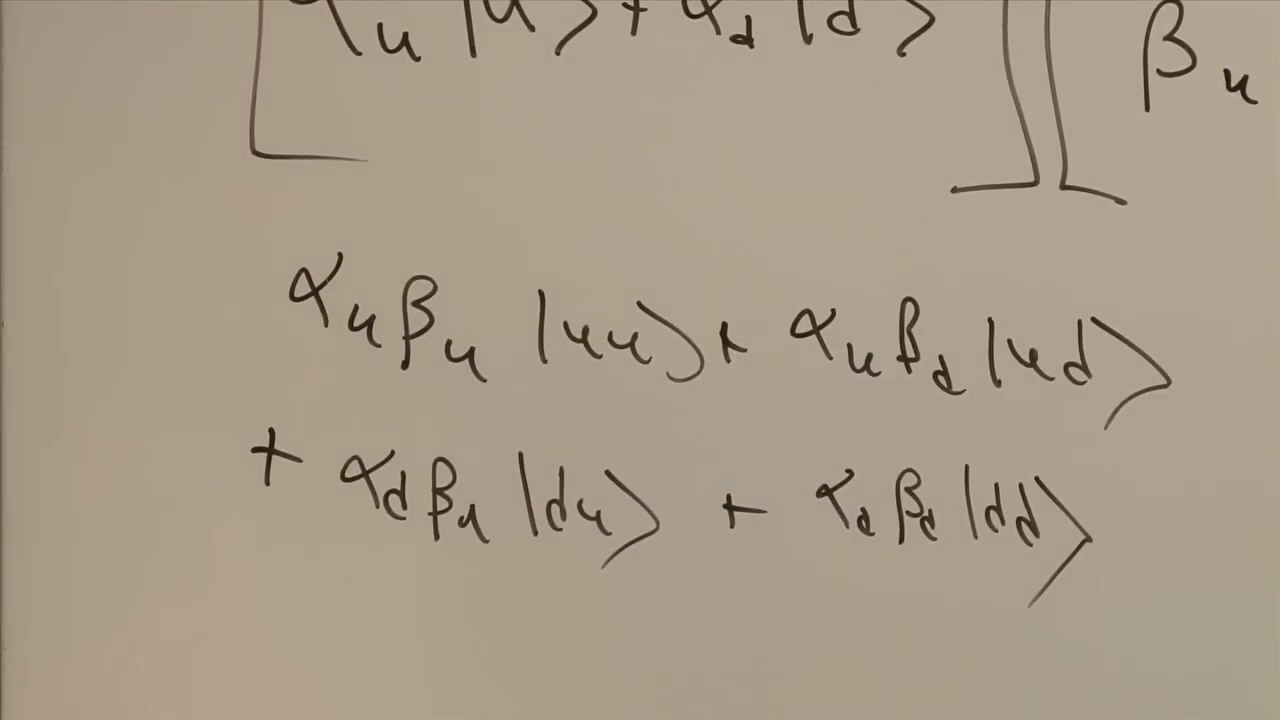
\includegraphics[width=0.86\textwidth]{lecture_06_figure_04.png}
\caption{一个在四态复合基中展开的因子化双自旋态。}
\lectureframe{00:37:45}
\end{figure}

\begin{classroomqa}
\audiencequestion{式~\eqref{eq:l6-product-expansion}中出现的是哪种矢量积？}
\lecturerresponse{所在的空间是两个希尔伯特空间的张量积。一个自身分解为分别来自这两个空间的一个矢量的矢量，称为乘积态或简单张量。张量积空间中的大多数矢量都是这种乘积的求和，不能写成单个乘积。}
\end{classroomqa}

这一限制可以直接从系数中看出：
\begin{equation}
c_{uu}c_{dd}=c_{ud}c_{du}
\qquad\text{for every product state}.
\label{eq:l6-rank-one-condition}
\end{equation}
等价地，\(2\times2\)系数矩阵的秩为1。参数计数也得出同样的结论。四个复系数包含八个实参数；归一化去掉一个，无关的整体相位再去掉一个，一般纯双自旋态还剩六个。每个纯单自旋态需要两个实参数，因此两个分别指定的自旋只需要四个。所以乘积态只占据六参数双自旋态空间中一个特殊的四参数子集。其余的状态是纠缠的。

\section{复合空间中的局域可观测量}

熟悉的自旋单粒子可观测量必须在更大的系统中继续存在。更明确地说，
\begin{equation}
\sigma_m\equiv\sigma_m\otimes I,
\qquad
\tau_n\equiv I\otimes\sigma_n,
\qquad
m,n\in\{x,y,z\}.
\label{eq:l6-local-operators}
\end{equation}
一旦固定了槽位约定，这种简写记号就无害了。使用
\begin{equation}
\begin{aligned}
\sigma_x&=
\begin{pmatrix}0&1\\1&0\end{pmatrix},\\[0.4em]
\sigma_y&=
\begin{pmatrix}0&-i\\i&0\end{pmatrix},\\[0.4em]
\sigma_z&=
\begin{pmatrix}1&0\\0&-1\end{pmatrix},
\end{aligned}
\end{equation}
第一个自旋的算符作用时，第二个标签是旁观者：
\begin{align}
\sigma_x\ket{u\,i}&=\ket{d\,i},
&
\sigma_x\ket{d\,i}&=\ket{u\,i},\\
\sigma_z\ket{u\,i}&=\ket{u\,i},
&
\sigma_z\ket{d\,i}&=-\ket{d\,i}.
\end{align}
对于第二个自旋，第一个标签是旁观者：
\begin{align}
\tau_x\ket{a\,u}&=\ket{a\,d},
&
\tau_x\ket{a\,d}&=\ket{a\,u},\\
\tau_z\ket{a\,u}&=\ket{a\,u},
&
\tau_z\ket{a\,d}&=-\ket{a\,d}.
\label{eq:l6-spectator-action}
\end{align}
\(y\)分量也会翻转其活动槽位，其中
\(\sigma_y\ket{u}=i\ket{d}\)且
\(\sigma_y\ket{d}=-i\ket{u}\)。

\begin{figure}[htbp]
\centering
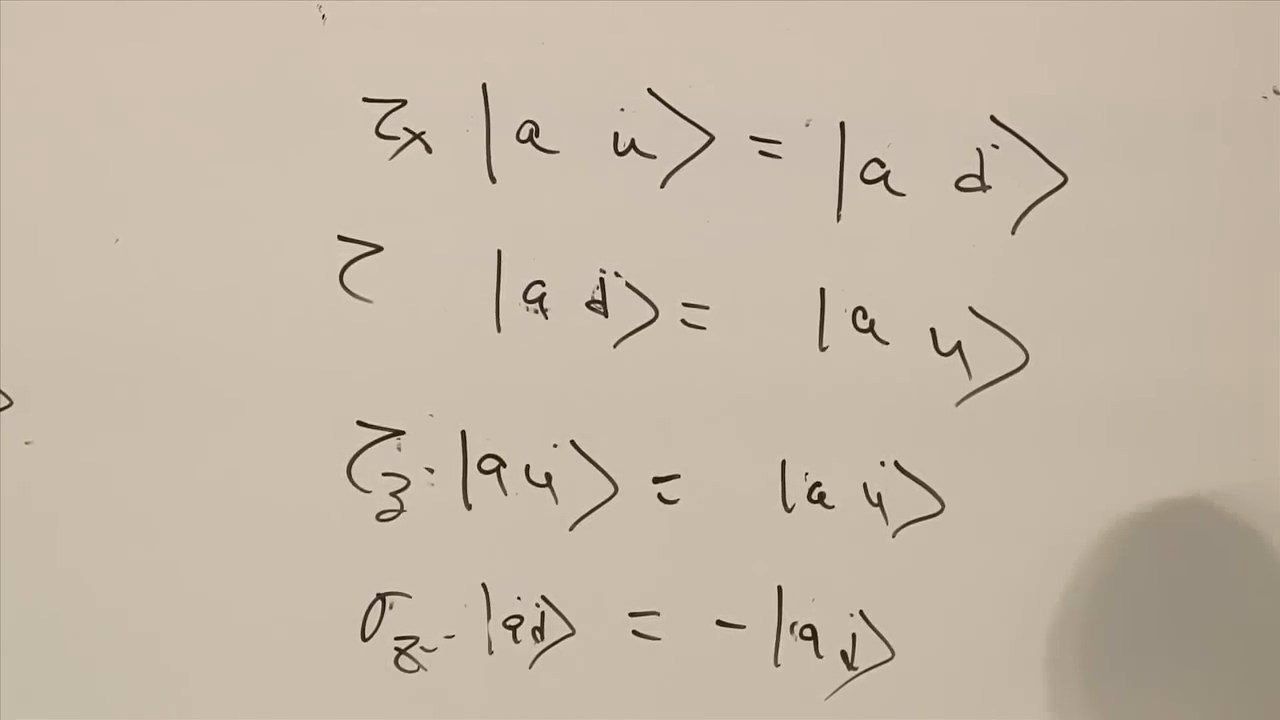
\includegraphics[width=0.86\textwidth]{lecture_06_figure_05.png}
\caption{第二个自旋的作用表：第一个指标保持为旁观者。}
\lectureframe{00:47:40}
\end{figure}

\begin{classroomqa}
\audiencequestion{施加\(\sigma_x\)是否意味着已经发生了一次\(x\)测量，为什么结果不是叠加态？}
\lecturerresponse{算符作用本身并不是测量。将矩阵\(\sigma_x\)乘以\(z\)基矢量\(\ket{u}\)得到\(\ket{d}\)。这不是本征值方程：本征矢量在算符作用下会保持其方向。确实，\(\ket{u}\)被映射到一个正交态，这是看出为什么对\(z\)本征态进行\(x\)测量会得到最大随机性的另一种方式。作用于非本征矢量通常只是一个中间代数步骤，其物理意义来自所计算的完整量。}
\end{classroomqa}

作用于不同因子的算符对易。例如，
\begin{equation}
\sigma_x\tau_x\ket{uu}
=\ket{dd}
=\tau_x\sigma_x\ket{uu}.
\end{equation}
同样的等式对每个复合基矢量都成立，因此对每个态都成立：
\begin{equation}
[\sigma_m,\tau_n]=0
\qquad\text{for all }m,n.
\label{eq:l6-local-commutation}
\end{equation}

\begin{figure}[htbp]
\centering
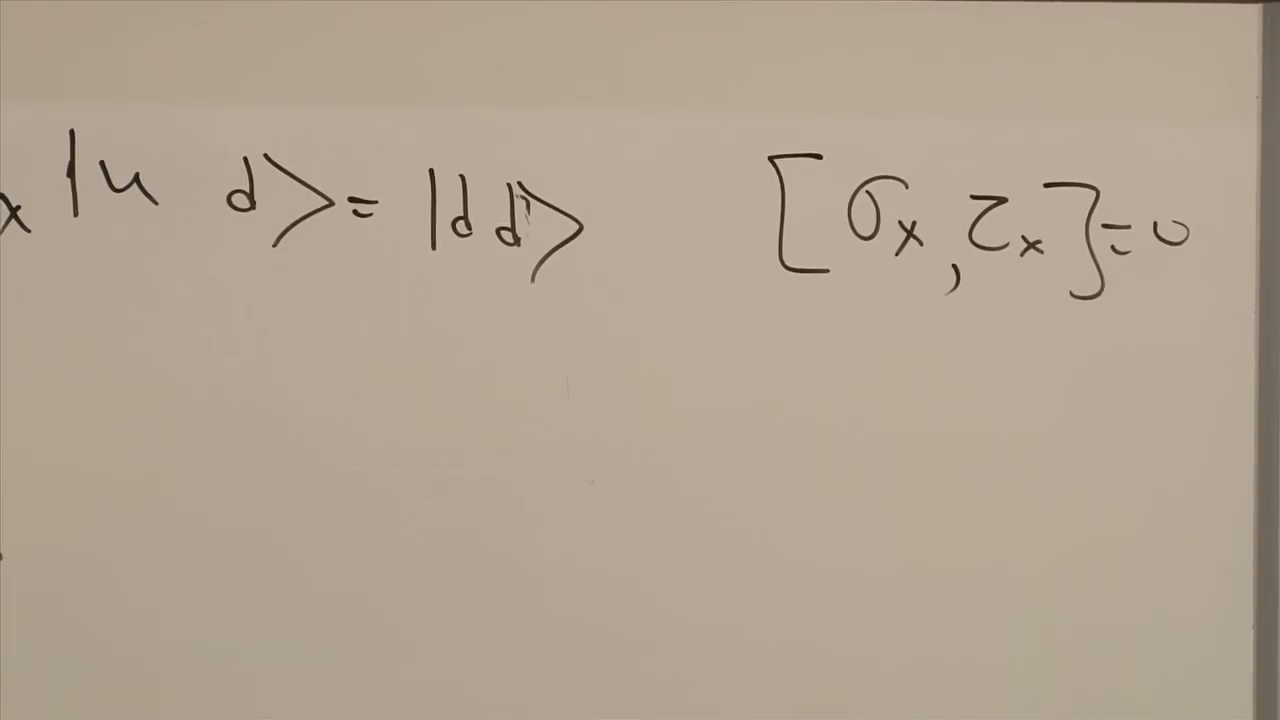
\includegraphics[width=0.86\textwidth]{lecture_06_figure_06.png}
\caption{分别作用于各自槽位导致对易子\([\sigma_x,\tau_x]\)为零。}
\lectureframe{00:56:40}
\end{figure}

\begin{classroomqa}
\audiencequestion{为什么检查一个基矢量还不能证明两个算符对易？}
\lecturerresponse{算符相等要求对每个矢量作用相同。只需检查一组基中的每个矢量就足够了，因为线性性随后会把结果推广到每个叠加态。对于局域算符，论证在全部四个基态上都是直接的：每个算符改变不同的槽位，所以它们的顺序无关紧要。}
\end{classroomqa}

\begin{classroomqa}
\audiencequestion{是否存在真正属于双自旋系统的可观测量？}
\lecturerresponse{是的。诸如\(\sigma_x\tau_x\)、\(\sigma_x\tau_y\)这样的乘积以及这类乘积的线性组合探测的是联合性质。局域可观测量描述每个因子；关联可观测量揭示各因子如何相互关联。}
\end{classroomqa}

\begin{classroomqa}
\audiencequestion{独立制备的乘积态已经纠缠了吗？}
\lecturerresponse{没有。在乘积态中，每个因子都有自己的态矢量，局域期望值因子化。当复合态不能分离为\(\sigma\)的一个态和\(\tau\)的一个态时，纠缠才开始。}
\end{classroomqa}

\section{单态}

一个最大纠缠的例子是
\begin{equation}
\ket{S}
=\frac{1}{\sqrt2}\bigl(\ket{ud}-\ket{du}\bigr).
\label{eq:l6-singlet}
\end{equation}
这两项已经显示出沿\(z\)的完美反关联：只要一个自旋向上，另一个就向下。更深层的要点是，两个自旋都不能被赋予自己的纯态。

\begin{figure}[htbp]
\centering
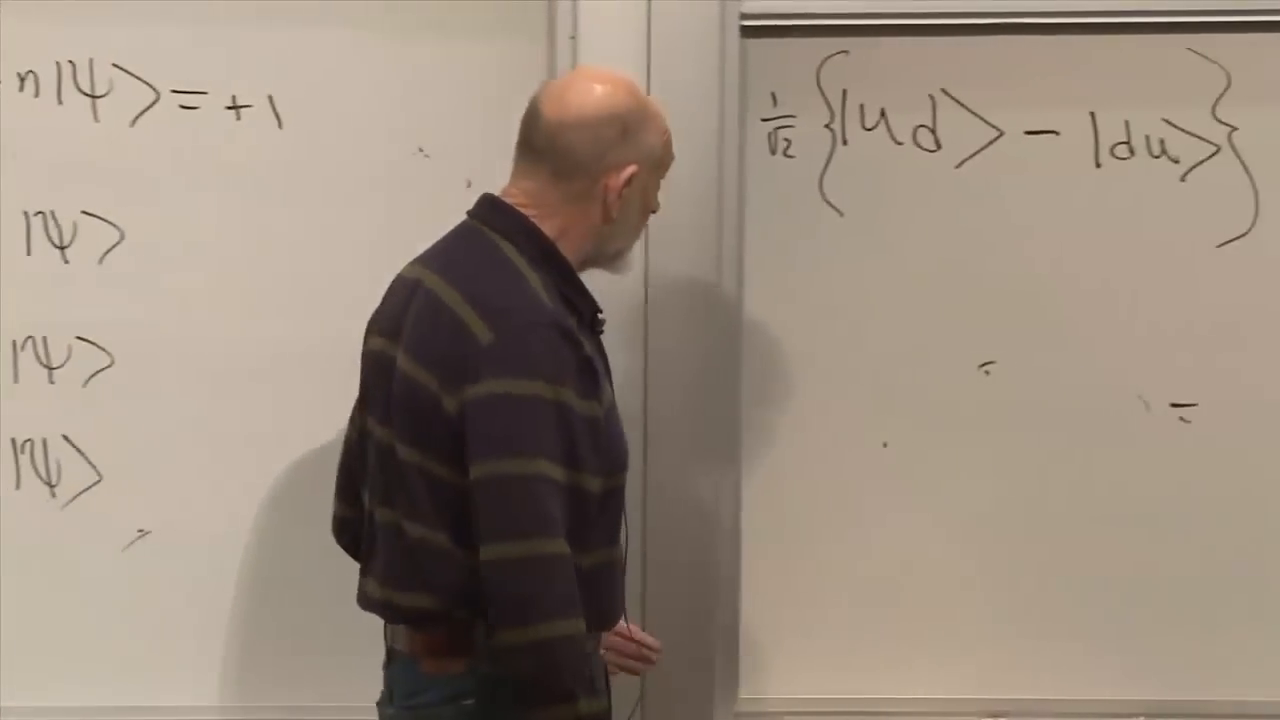
\includegraphics[width=0.86\textwidth]{lecture_06_figure_07.png}
\caption{将被认定为单态的反对称双自旋态。}
\lectureframe{01:09:25}
\end{figure}

对于单个自旋的纯态，总存在一个单位矢量\(\bm n\)使得
\begin{equation}
(\bm\sigma\cdot\bm n)\ket{\psi}=\ket{\psi}.
\end{equation}
等价地，Bloch矢量
\begin{equation}
\bm r
=\bigl(\expect{\sigma_x},\expect{\sigma_y},\expect{\sigma_z}\bigr)
\end{equation}
对于单自旋纯态长度为1。因此它的三个分量不可能全部为零。给定该态，将探测器沿\(\bm r\)取向会以确定性得到\(+1\)。熟悉的例子是：对于\(\ket{u}\)为\(z\)，对于\((\ket{u}+\ket{d})/\sqrt2\)为\(x\)，对于\((\ket{u}+i\ket{d})/\sqrt2\)为\(y\)方向之一。

现在计算单态中的一个局域平均值：
\begin{align}
\expect{\sigma_z}_S
&=\frac12
(\bra{ud}-\bra{du})\sigma_z
(\ket{ud}-\ket{du})\\
&=\frac12
(\bra{ud}-\bra{du})
(\ket{ud}+\ket{du})\\
&=0.
\end{align}
对于\(\sigma_x\)，
\begin{equation}
\sigma_x\ket{S}
=\frac{\ket{dd}-\ket{uu}}{\sqrt2},
\end{equation}
它与\(\ket{S}\)正交，所以\(\expect{\sigma_x}_S=0\)。由\(\sigma_y\)提供的相位不改变这种正交性，因此
\begin{equation}
\expect{\sigma_x}_S
=\expect{\sigma_y}_S
=\expect{\sigma_z}_S=0.
\label{eq:l6-zero-local-sigma}
\end{equation}
由对称性，
\begin{equation}
\expect{\tau_x}_S
=\expect{\tau_y}_S
=\expect{\tau_z}_S=0.
\label{eq:l6-zero-local-tau}
\end{equation}

\begin{figure}[htbp]
\centering
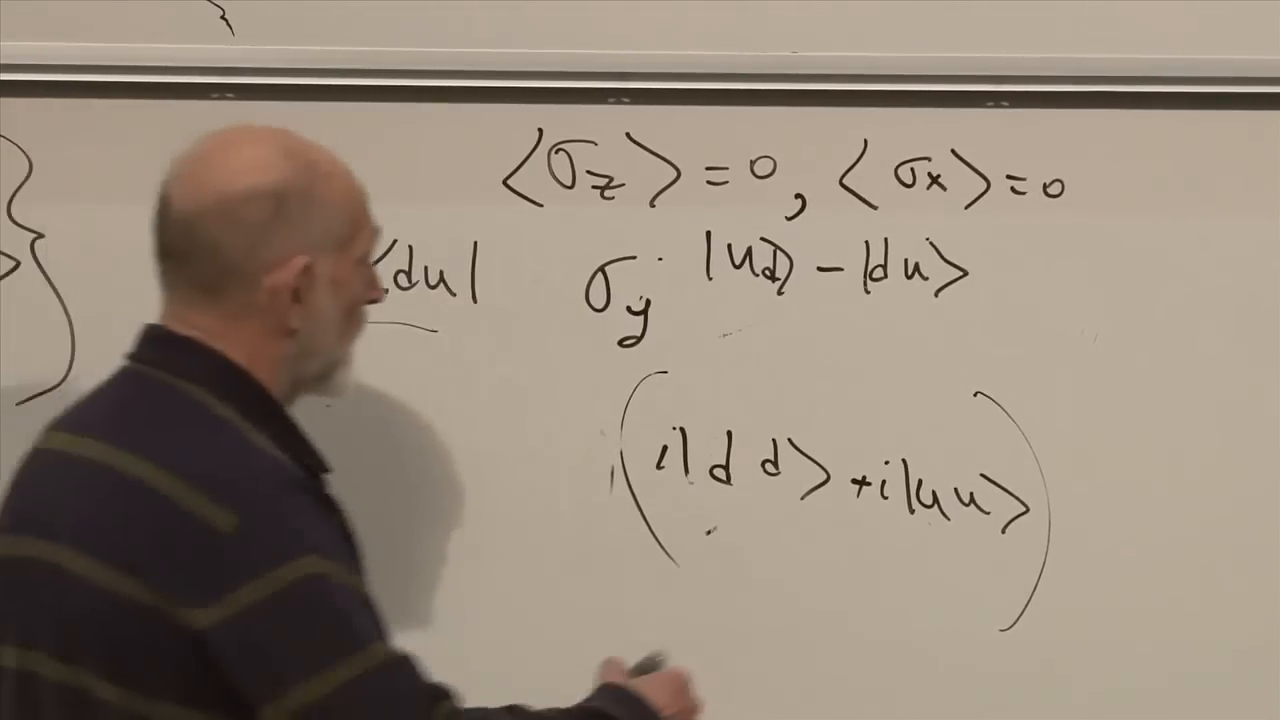
\includegraphics[width=0.86\textwidth]{lecture_06_figure_08.png}
\caption{板书记录了局域自旋平均值消失以及用于完成检验的\(y\)分量翻转。}
\lectureframe{01:14:20}
\end{figure}

整个双自旋态是纯态且完全已知，但每个部分在局域上都是未极化的。由于没有单自旋纯态具有零Bloch矢量，\(\ket{S}\)不可能是乘积态。

\begin{classroomqa}
\audiencequestion{普通乘积态是否仍然会有一个具有非零局域极化的方向？}
\lecturerresponse{是的。单自旋的证明适用于相关因子，而另一个因子只是旁观者。因此纯乘积态的每个因子都有一个单位Bloch矢量。单态对两个自旋都不满足这个乘积态性质。}
\end{classroomqa}

\begin{classroomqa}
\audiencequestion{如何将两个自旋制备到单态？}
\lecturerresponse{一种倾向于反平行的耦合可以使单态成为能量最低的状态。让两个自旋发生相互作用，并允许该对自旋向周围环境释放能量；它可以弛豫到单态。这一陈述取决于相互作用。对于各向异性反铁磁哈密顿量\(H_{\rm int}=J\,\bm\sigma\cdot\bm\tau\)，其中\(J>0\)，单态位于三个三重态之下。}
\end{classroomqa}

\begin{classroomqa}
\audiencequestion{这种弛豫需要多长时间？}
\lecturerresponse{时间尺度取决于两个自旋的间距、它们相互耦合的强度、它们的磁矩，以及它们与带走能量的电磁环境的耦合。耦合越强，通常意味着弛豫越快。}
\end{classroomqa}

\begin{classroomqa}
\audiencequestion{为什么反对称组合的能量可以低于对称组合？}
\lecturerresponse{对于两个自旋\(\tfrac12\)粒子，反对称态的总自旋为零，而三个对称态构成总自旋为一的三重态。正比于\(+\bm\sigma\cdot\bm\tau\)的相互作用给单态赋予本征值\(-3\)，给三重态赋予\(+1\)，因此正耦合使单态位置更低。其他哈密顿量未必以相同方式排列能级。}
\end{classroomqa}

\subsection{每个自旋基中的同一态}

选择更方便的局域基并不会消除纠缠。稍后发展的一个与基无关的度量是纠缠熵。单态展现出更强的对称性。将
\begin{equation}
\ket{u}=\frac{\ket{R}+\ket{L}}{\sqrt2},
\qquad
\ket{d}=\frac{\ket{R}-\ket{L}}{\sqrt2},
\end{equation}
代入方程~\eqref{eq:l6-singlet}得到
\begin{equation}
\ket{S}
=\frac{\ket{LR}-\ket{RL}}{\sqrt2}.
\label{eq:l6-singlet-x-basis}
\end{equation}
在任何共同的幺正自旋基\(\{\ket{\rm in},\ket{\rm out}\}\)中，
\begin{equation}
\ket{S}
=\frac{\ket{{\rm in}\,{\rm out}}-\ket{{\rm out}\,{\rm in}}}{\sqrt2},
\label{eq:l6-singlet-any-basis}
\end{equation}
直至一个无关紧要的整体相位。三个三重态在共同旋转下彼此混合；一维单态扇区只能再现自身。

\begin{figure}[htbp]
\centering
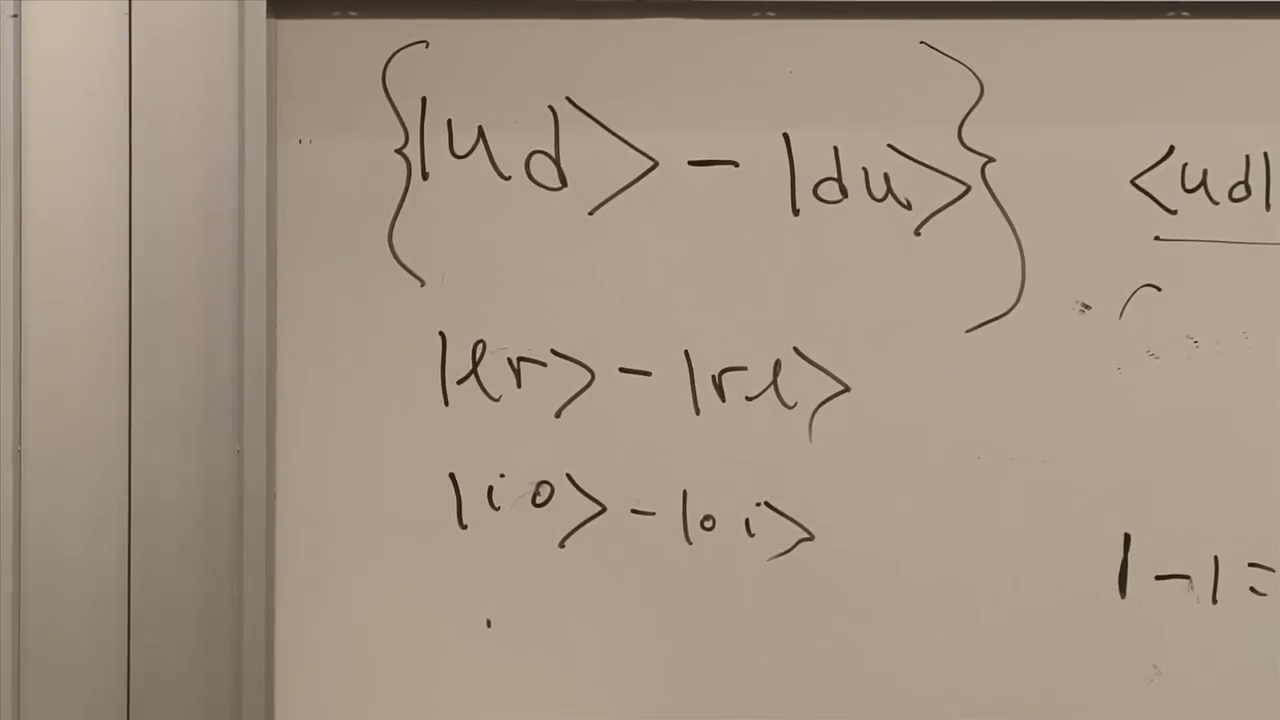
\includegraphics[width=0.86\textwidth]{lecture_06_figure_09.png}
\caption{反对称模式在从上下到左右以及其他共同自旋基的变化下保持不变。}
\lectureframe{01:21:00}
\end{figure}

\begin{classroomqa}
\audiencequestion{纠缠仅仅是用于写出该态的基的产物吗？}
\lecturerresponse{不是。局域基的改变会改变系数，但不会改变该态是否因子化，而纠缠熵量化了这一不变的事实。对于单态，共同旋转使这种不变性尤其明显：反对称形式在每个自旋基中都被再现。}
\end{classroomqa}

\section{关联可观测量}

局域平均值消失，因此单态中的信息必定存在于联合可观测量中。从
\begin{equation}
\sigma_z\tau_z\ket{ud}=-\ket{ud},
\qquad
\sigma_z\tau_z\ket{du}=-\ket{du}.
\end{equation}
开始，因此
\begin{equation}
\sigma_z\tau_z\ket{S}=-\ket{S},
\qquad
\expect{\sigma_z\tau_z}_S=-1.
\label{eq:l6-zz-correlation}
\end{equation}
这一结果不仅仅是一个平均值：单态是该乘积的本征态，因此同轴\(z\)测量总是具有相反的符号。

两个\(x\)算符都翻转它们的槽位：
\begin{equation}
\sigma_x\tau_x\ket{ud}=\ket{du},
\qquad
\sigma_x\tau_x\ket{du}=\ket{ud}.
\end{equation}
交换这两项会反转反对称态：
\begin{equation}
\sigma_x\tau_x\ket{S}=-\ket{S},
\qquad
\expect{\sigma_x\tau_x}_S=-1.
\end{equation}
来自\(y\)算符的两个相位以相同方式相消，给出
\begin{equation}
\expect{\sigma_y\tau_y}_S=-1.
\end{equation}
相比之下，不相等的笛卡尔分量具有零期望值。例如，
\begin{equation}
\sigma_x\tau_z\ket{S}
=-\frac{\ket{dd}+\ket{uu}}{\sqrt2},
\qquad
\expect{\sigma_x\tau_z}_S=0.
\end{equation}
所有这些结果总结为
\begin{equation}
\expect{\sigma_m\tau_n}_S=-\delta_{mn},
\qquad
\expect{(\bm\sigma\cdot\bm a)(\bm\tau\cdot\bm b)}_S
=-\bm a\cdot\bm b.
\label{eq:l6-singlet-correlation-tensor}
\end{equation}

\begin{figure}[htbp]
\centering
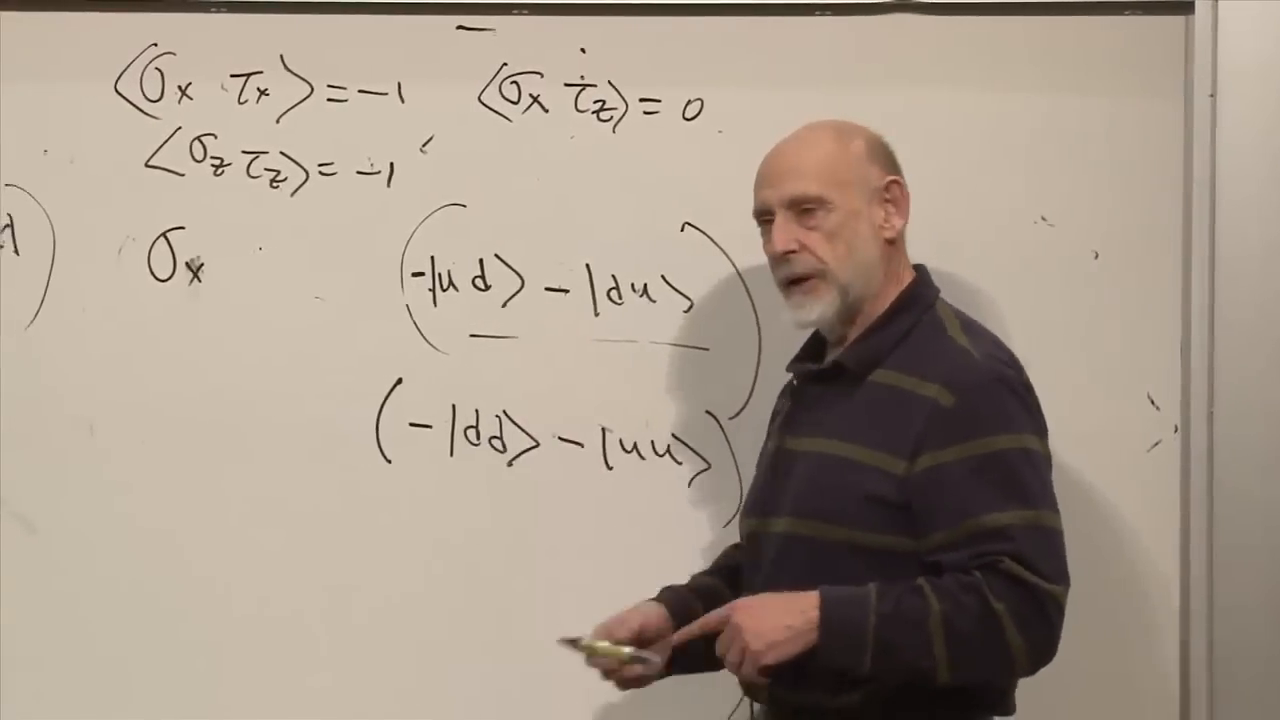
\includegraphics[width=0.86\textwidth]{lecture_06_figure_10.png}
\caption{关联计算记录了\(\expect{\sigma_x\tau_x}=-1\)和混合轴结果\(\expect{\sigma_x\tau_z}=0\)。}
\lectureframe{01:32:20}
\end{figure}

\begin{classroomqa}
\audiencequestion{两个可观测量的乘积在物理上意味着什么？是一次测量在另一次之后进行吗？}
\lecturerresponse{一般来说，厄米乘积是复合空间上的另一个可观测量。这里每个\(\sigma_m\)都与每个\(\tau_n\)对易，因此两个局域分量可以同时测量，并将它们的数值结果相乘。乘积算符打包了这一联合结果；不需要时间顺序。}
\end{classroomqa}

对于乘积态，联合平均值因子化：
\begin{equation}
\expect{\sigma_m\tau_n}_{\rm prod}
=\expect{\sigma_m}_{\sigma}\expect{\tau_n}_{\tau}.
\end{equation}
单态最大程度地违反这种因子化。右边的每个因子都会是零，而左边的同轴乘积是\(-1\)。单独来看，两个自旋完全随机；联合来看，相等的分量必定相反。

\begin{classroomqa}
\audiencequestion{两个自旋之间的每一种相互作用都会产生纠缠吗？}
\lecturerresponse{一般的耦合可以使初始因子化的态纠缠，许多普通相互作用都会如此。这并非字面意义上的必然：一个特别选择的乘积本征态可能只获得一个相位，而纯局域哈密顿量不能使因子纠缠。重要的是一个非平凡耦合作用于一个它并不作为乘积保持的态。}
\end{classroomqa}

\section{从关联到贝尔的问题}

完美的反关联本身并不悖谬。设想把一枚便士和一枚角币放进衣袋，将其中一枚未露面的硬币分给爱丽丝，另一枚分给鲍勃，再把它们送到相距很远的地方。当爱丽丝看到自己拿到的是哪一枚硬币时，她立刻就知道鲍勃的硬币是哪一枚。这种关联是在两枚硬币还在一起时建立起来的；得知一个结果并不会向另一处发送任何信号。

单态也具有这一基本特征，但增加了一个关键的自由度：爱丽丝和鲍勃可以选择任意测量方向，而量子力学预言了连续变化的关联\(-\bm a\cdot\bm b\)。贝尔定理要问的是，所有这些关联是否都能由粒子事先携带的局域经典指令产生。

\begin{classroomqa}
\audiencequestion{这是贝尔定理中所用的态吗？}
\lecturerresponse{是的。贝尔型论证使用的是像单态这样的纠缠对，而不是确定的乘积态\(\ket{ud}\)。这一区分很重要，因为乘积态提供的是各自独立的局域描述，而单态则在每一个共同基上都携带一种不可分离的关联结构。}
\end{classroomqa}

\begin{classroomqa}
\audiencequestion{既然沿相同轴的结果总是相反，为什么还说这种反关联是统计性的？}
\lecturerresponse{每个局域结果都是随机的：爱丽丝无法预知自己会得到\(+1\)还是\(-1\)。条件关系则是精确的：一旦已知沿相同轴的一个结果，另一个结果就被确定为相反。关联指的是联合分布，而不是沿相同轴乘积中的不确定性。}
\end{classroomqa}

把问题说得更清楚的一个有用办法是通过模拟。一台经典计算机就能模仿关于一个自旋的每一个实验：存储它的态，用Schr\"odinger方程演化它，计算所要求的概率，并用随机数发生器选出一个结果。重复测量和磁进动都可以被再现。

现在把一对纠缠粒子分给两台经典计算机。允许这两台计算机在这对粒子被制备期间相互作用，然后把它们断开，并在相距遥远的地点独立选择测量方向。任何一对分离的局域经典程序，即使事先固定了共享随机性，也无法对每一种方向选择都再现量子关联。全局的经典模拟是可能的，但它必须保持对联合态的访问，或者以某种并非局域隐变量模型的方式协调两侧。

这种局域经典记账方式的失败并不提供超光速通信信道。爱丽丝的局域结果仍然是随机的，因此她无法控制一条鲍勃无需事后比对双方记录就能读出的消息。围绕非定域性的术语各不相同，但操作上的区分是明确的：贝尔关联排除了局域经典解释，同时保持了无信号性。

因此，复合态的构造产生了某种真正新的东西。张量积在局域上保留了旧有的单自旋物理，然而它们的一般向量却无法被分解为各自独立的态。在单态中，所有局域极化都消失，而联合自旋分量却携带完美的、与基无关的反关联。下一步就是要把这一结构转化为贝尔对经典推理的定量检验。
